\part{Models of Data}
With a solid development of the model of process that will be used to
represent the consistency of varied epidemiological rates as disease
moves through a population, I now turn to modeling the
epidemiological rate data collected in a systematic review of the
available data.  There are three parts to this model, treated in turn:
models for the stochastic variation, models for the heterogeneous age
groups found in systematic review, and models for the non-sampling
variation.

A useful theoretical framework to guide the development of
meta-regression techniques is to consider how the model would proceed
if, for each and every study identified in systematic review, complete
microdata were available.  Of course, it is unusual that microdata are
available for even \emph{one} study from the systematic review.  But
if all of the microdata were available, say for all of the prevalence
studies conducted on schizophrenia (an example I will return to in
the next section), modeling could proceed through standard techniques
for analyzing binary data, such as logistic or probit regression, with
fixed effects to explain some of the non-sampling variation, such as
differing diagnostic criteria, and random effects to model the
additional non-sampling variation, such as inherent differences
between populations (if they exist).

Viewed in this light, the task of a meta-regression model is to
produce the results that would be obtained from an analysis of the
full microdata, if they were available. The approach that will be
developed below decomposes into three parts: the epidemiological rate
model, which captures the sampling error in systematic review data;
the age-interval model, which addresses the heterogeneity of age
groups reported in the literature; and the covariate model, which
models the non-sampling variation between different sources of data
through fixed and random effects.

\chapter{Statistical Models for Rates, Ratios, and Durations}
\label{theory-rate_model}

The key to connecting the systems dynamics model from
Chapter~\ref{theory-system_dynamics} to the evidence base collected
through systematic review is the \emph{data model}.  This is a
statistical model, which has its core features defined by its
likelihood function.  By \emph{likelihood function}, I mean a
probability density function that assigns a value for the likelihood
of every possible observed value, for any setting of the model
parameters.

An example will make this clearer, so I turn now to the meta-analysis
of population prevalence of schizophrenia in adult males.  Strictly
speaking, prevalence is a ratio, not a rate, although in the
literature the term ``prevalence rate'' is often used to mean
prevalence ratio.  The prevalence of a condition in a population says
something about the stocks in the stock-and-flow model from
Chapter~\ref{theory-system_dynamics}: for a specific time period and
age group, prevalence is the ratio of individuals with the condition
to individuals in the population.

The forest plot in Figure~\ref{rate-model-schiz-forest} shows the
results of combining $16$ studies using $7$ different data models.  As
the figure demonstrates, the choice of data model can have a huge
effect on the estimated uncertainty, and can have a noticeable effect
on the estimated median as well. The models I displayed produce point
estimates ranging from $1.2$ to $4.0$ per thousand, and uncertainty
intervals with widths ranging from $0.1$ to $2.9$.  Clearly, the
choice of data model influences the estimate.

\begin{figure}[h]
\begin{center}
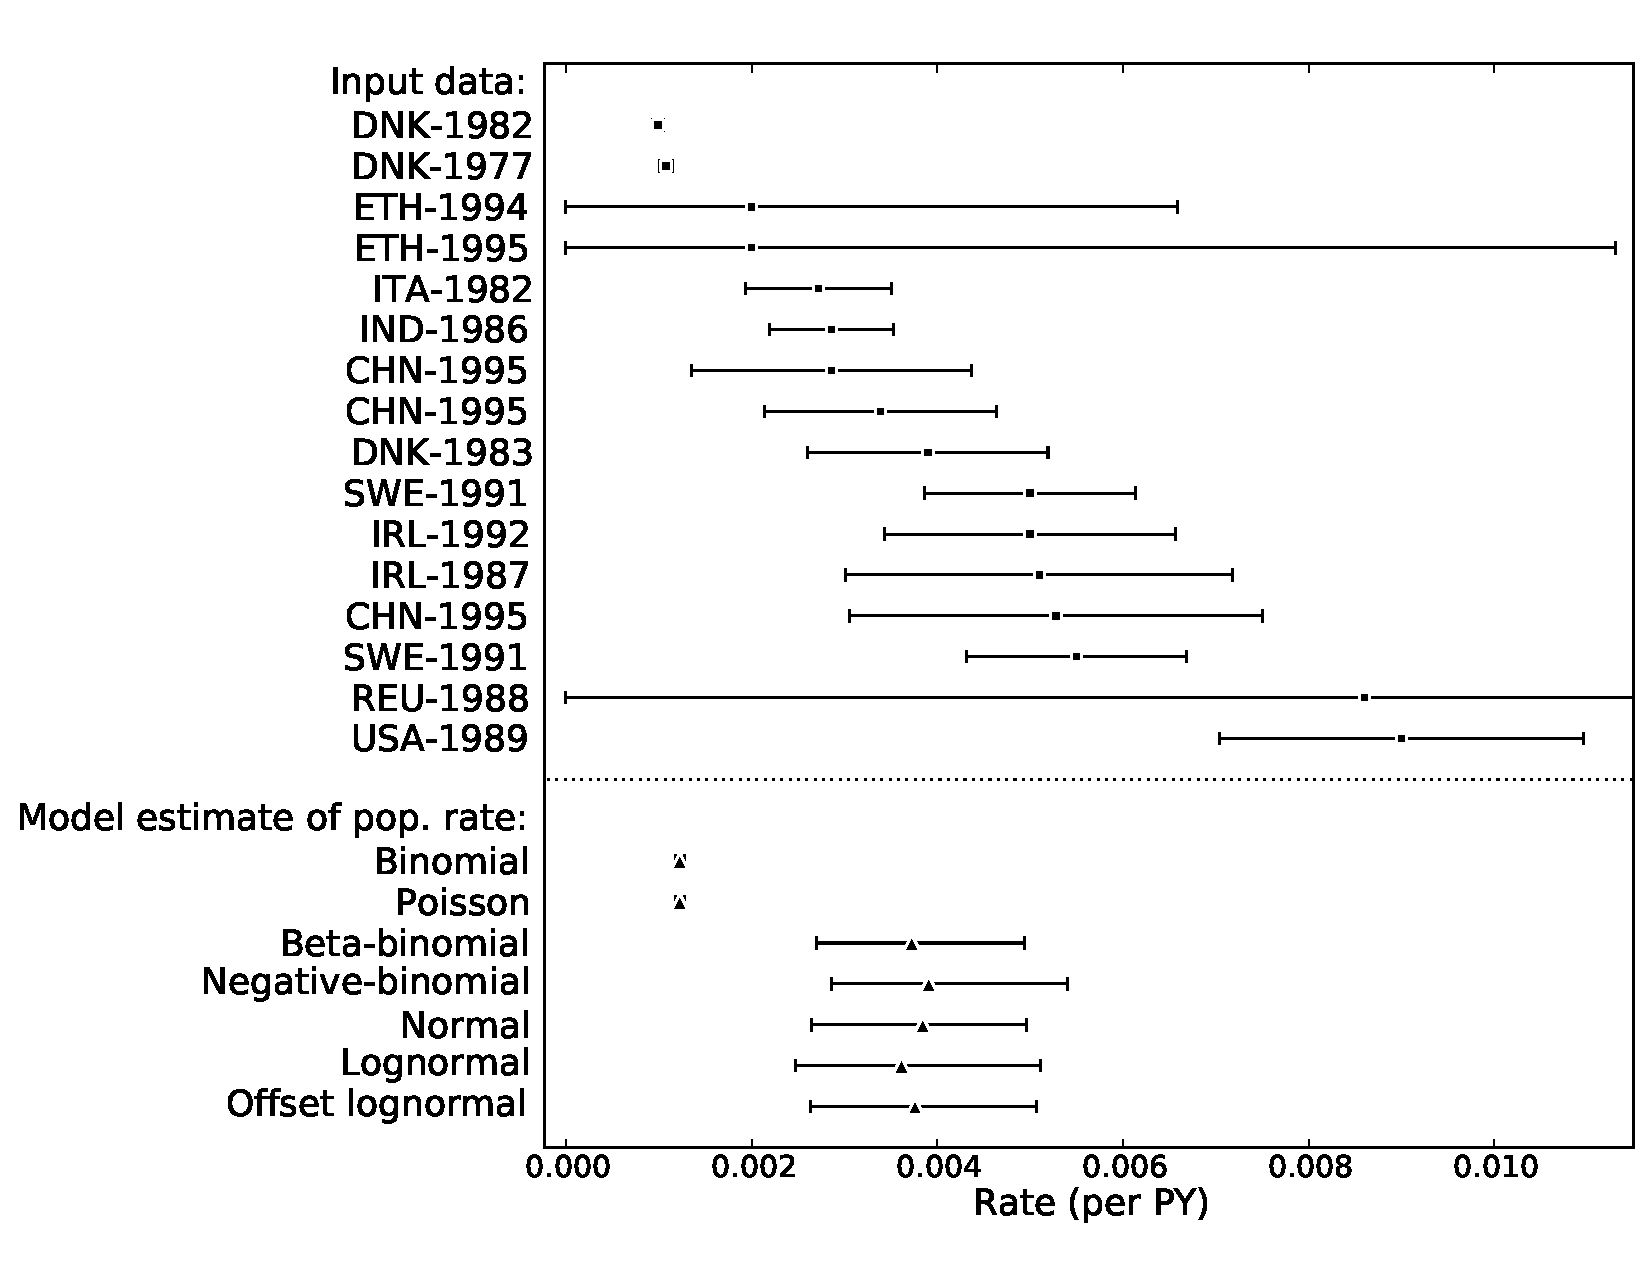
\includegraphics[width=\textwidth]{schiz_forest.pdf}
\caption{Forest plot summarizing $7$ alternative models for
  meta-analysis of adult male schizophrenia prevalence at
  population-level.  The median estimates range from
  $1.2$ to
  $4.0$ per thousand person years, and the width of the
  $95\%$ HPD interval ranges from
  $0.1$ to
  $2.9$.}
\label{rate-model-schiz-forest}
\end{center}
\end{figure}

In what follows, I will develop a collection of data models, starting
with the simplest and then increasing the complexity, while
identifying the benefits and drawbacks of each.  The models to come,
in order, are the binomial model, the beta-binomial model, the Poisson
model, the negative binomial model, and three variants of the normal
model.

\section{Binomial Model}
Conceptually, the simplest model I consider for epidemiological data
is built from the binomial random variable. Random variable $X$ is
\emph{binomially distributed} if it has probability distribution
\[
\Pr[X=k\given n, \pi] = \binom{n}{k}\pi^n(1-\pi)^{n-k}
\]
for some $\pi$.  I've used greek to emphasize that $\pi$ is a model
parameter, while $n$ and $k$ are data.

Although this equation may appear opaque, the intuition behind it is
simple: $n$ individuals were tested for a disease, and $k$ tested
positive. The formula then follows from the assumption that each
individual tested positive with probability $\pi$, and that if I know
$\pi$, then knowing about the test results of any subset of
individuals gives me no information about the test results for the
others (these events are ``independent'').

The intuitive description in the previous paragraph is particularly
relevant to a study that measures the \emph{prevalence} of a disease
in a population.  Strictly speaking, prevalence is a \emph{ratio} not
a rate.  It is a unitless metric, often expressed as a fraction or a
percentage.  Incidence, remission, and mortality rates, on the other
hand, are \emph{rates}, measured per unit time.  For example,
incidence is often expressed in the units of ``per person-year'' or
``per 1000 person-years''.  Nonetheless the binomial distribution can
be the basis of a statistical model for rates as well as for
prevalence.  I will argue that it is not a very good model, and the
fact that, in its intuitive description, it has the wrong units is
only one of its shortcomings.  I believe that it is instructive to
begin with simple models and make them more complicated, until they
are just complicated enough.

The binomial distribution inspires a computationally tractable
data model for an observed population prevalence of
$p$ in a sample population of size $n$:
\[
\dens(p\given \pi, n) \propto \pi^{\lfloor pn \rfloor}(1-\pi)^{\lceil (1-p)n \rceil}.
\]
Here $\lfloor \cdot \rfloor$ is the ``floor'' operator, which rounds
real numbers down to the largest integer less than or equal to the
operand, and $\lceil \cdot \rceil$ is the ``ceiling'' operator, which
rounds up.

Note that it is not necessary to include the normalization term
$\binom{n}{\lfloor np\rfloor}$, because this does not depend on the
model parameter $\pi$. This constant of proportionality is necessary
to make this data model truly a probability density function for any
$\pi$ and $n$. But I will never need to know this constant, and I use
the ``proportional to'' symbol $\propto$ instead of equality to
emphasize this fact.

The funnel plot in Figure~\ref{rate-model-binom-funnel} shows the
predictive distribution of this rate model for $\pi=.004$.  It also
shows the potential problem with this approach: the data gathered by
systematic review are often much more dispersed than this distribution
predicts.

\begin{figure}[ht]
\begin{center}
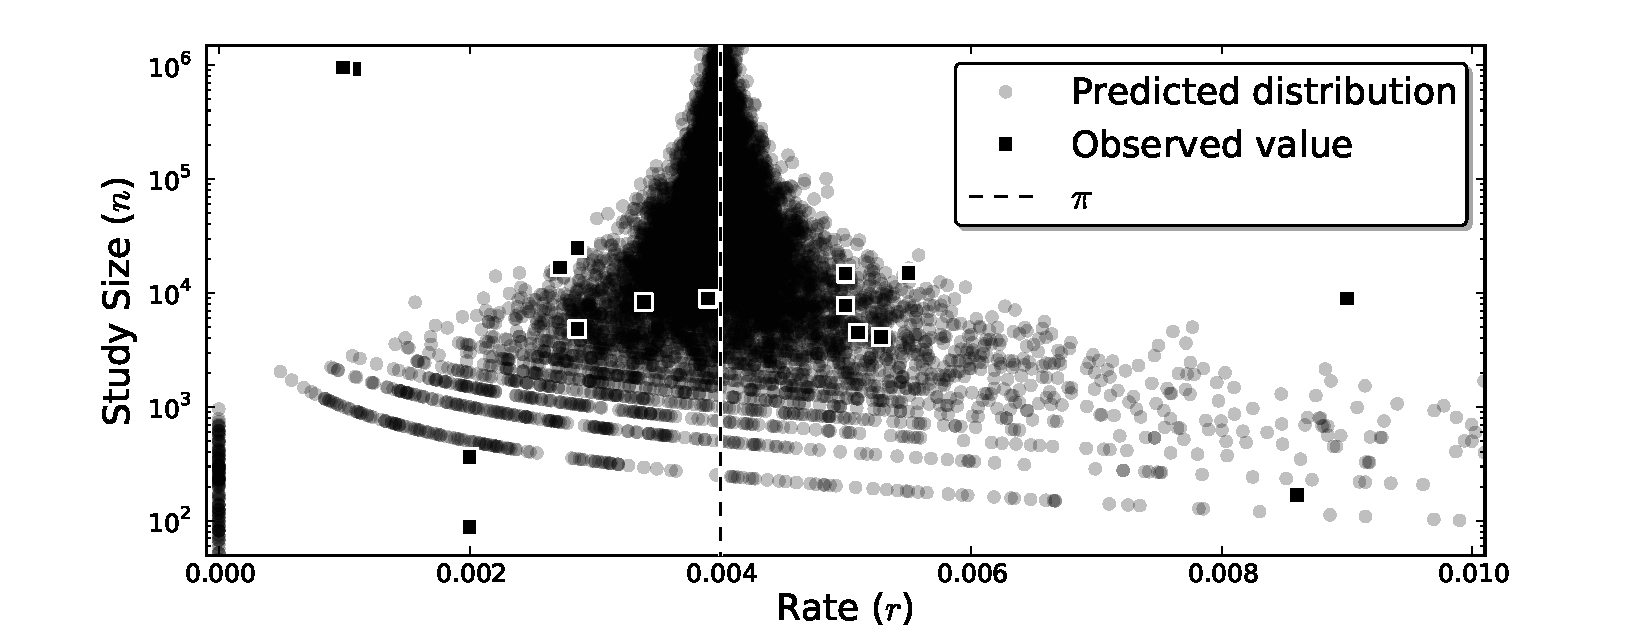
\includegraphics[width=\textwidth]{binomial-model-funnel.pdf}
\end{center}
\caption{Funnel plot showing predictive distribution for the binomial
  rate model with $\pi=.004$ (samples from this distribution are
  marked by circles), with data from systematic review for adult male
  schizophrenia prevalence overlaid for comparison (observations
  marked by squares).}
\label{rate-model-binom-funnel}
\end{figure}

All models are wrong, of course, so why does this model require
refinement? The answer is that it leads to unreasonably high
confidence when modeling noisy data.  It does so because it does not
account sufficiently for noise in the measurement of $p$. If a study
of $50,000$ people from subpopulation A finds prevalence of $2$ per
thousand and a study of the same size in subpopulation B finds $6$ per
thousand, then the binomial model predicts that a third study
conducted in subpopulation C will have prevalence of $4$ per thousand,
with $95\%$ HPD interval $[3,5]$.  I have no problem with the point
estimate; picking the mean of the two populations seems just right.
But the uncertainty interval lacks face validity.  It would be much
more reasonable to have an uncertainty interval as large as $[1,7]$,
instead of one as small as this.

One way to formalize this objection is through the posterior
predictive check, an in-sample goodness-of-fit test that graphically
compares the observed data to the \emph{posterior predicted
  distribution}, which is to say the model's prediction for what the
data should be, after it has been fit to the data \cite{Gelman book or
  paper}.  Figure~\ref{rate-model-binom-ppc} shows $1,000$ draws from
the posterior predicted distribution for each of the data
observations, together with the observation itself.  The model
predictions are compressed, showing a cloud of predicted points that
often does not include the observation.  Trusting the results of such
a model leads to inappropriately high certainty about the nature of
this noisy data.

\begin{figure}[ht]
\begin{center}
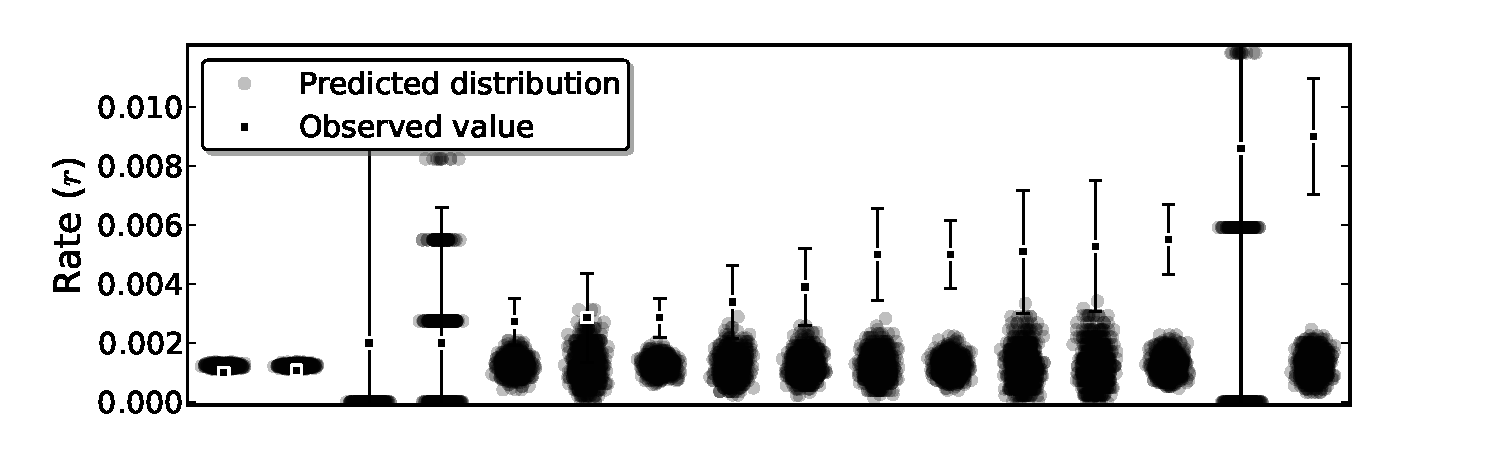
\includegraphics[width=\textwidth]{binomial-model-ppc.pdf}
\caption{Posterior predictive check for binomial model fit to adult
  male schizophrenia data.  Circular markers shows $1,000$ draws from
  the posterior distribution of the binomial model, and square markers
  show the observed data.  The confidence interval marked by error
  bars around each square shows the sampling error for each
  observation, based on the sample size alone. More than half of the
  data observations fall outside the posterior predicted distribution
  samples, indicating that the model is not capturing the
  heterogeneity observed in the data.}
\label{rate-model-binom-ppc}
\end{center}
\end{figure}


\section{Beta-binomial model}
\label{beta-binomial-model}
A theoretically appealing extension to the binomial model (which also
is not sufficient for my purposes) is the beta-binomial model.  I will
develop it in this section, to motivate the following sections.

Formally, a beta-binomial random variable $X$ has the following
probability distribution
\begin{align*}
\Pr[X = k\given n, \alpha, \beta]  &= \int_{\pi=0}^1 \dens(\pi\given \alpha, \beta) \binom{n}{k}\pi^k(1-\pi)^{n-k} d\pi\\
\dens(\pi\given \alpha, \beta) &\propto \pi^{\alpha-1}(1-\pi)^{\beta-1}
\end{align*}

The intuition behind this model is simpler than the equation,
however. As in the binomial model, each individual tests positive for
the condition independently with a probability $\pi$, but now $\pi$
itself is a random variable, distributed according to a beta
distribution with parameters $\alpha$ and $\beta$. The beta
distribution is given by 
\[
\dens(\pi\given \alpha, \beta)
\propto \pi^{\alpha-1}(1-\pi)^{\beta-1}
\]
and has a high degree of flexibility.  It also always takes values
between zero and one, making it an appropriate distribution for a
probability.  Figure~\ref{rate-model-beta} shows the probability
density of the beta distribution for several combinations of $\alpha$
and $\beta$.
\begin{figure}[ht]
\begin{center}
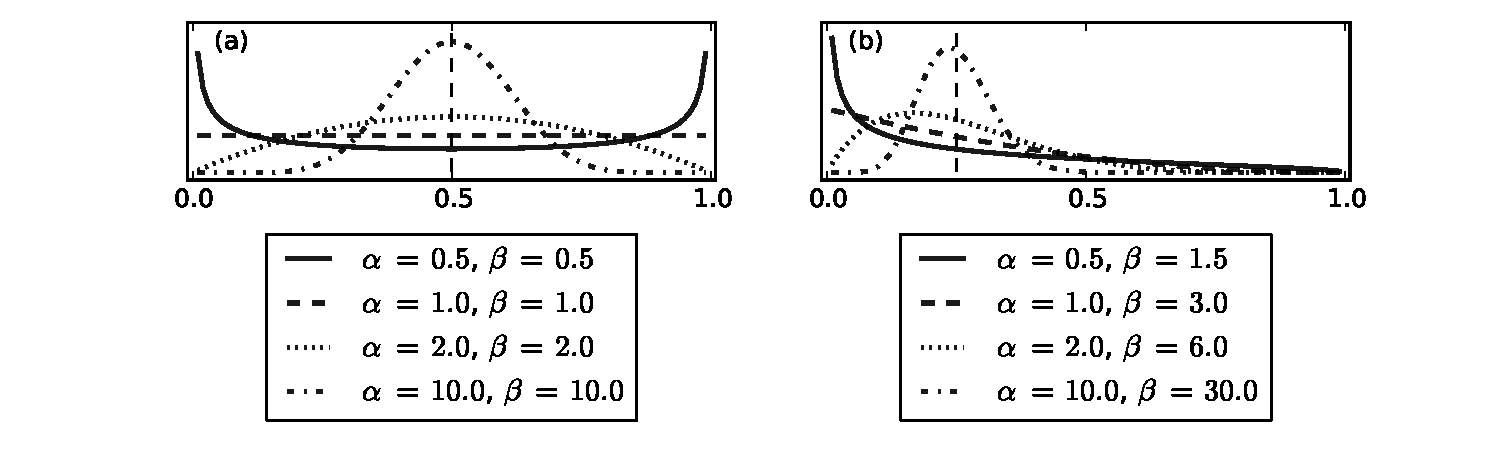
\includegraphics[width=\textwidth]{beta-distribution.pdf}
\end{center}
\caption{Probability density for the beta distribution for a range of
  $\alpha$ and $\beta$ values. Dashed black line shows expected value,
  which is $\frac{1}{2}$ for all distributions in Panel~(a) and
  $\frac{1}{4}$ for all in Panel~(b).}
\label{rate-model-beta}
\end{figure}

The beta binomial distribution inspires the following data model for
an observed prevalence of $p$ in a population of size $n$:
\[
\dens(p\given \alpha, \beta, n) \propto 
\int_{\pi=0}^1 \pi^{\alpha-1}(1-\pi)^{\beta-1}
\pi^{\lfloor pn\rfloor} (1-\pi)^{\lceil (1-p)n\rceil} d\pi.
\]

This model extends the binomial model in a way analogous to a random
effects model in linear regression.  By introducing additional
dimensions into the parameter space, the model is able to capture the
dispersion beyond the binomial model that I have observed empirically
in funnel plots of real data
(Figure~\ref{rate-model-beta-binomial-funnel} shows the beta
binomial funnel plot, as well as the posterior predictive check for
this model on the same data as used in
Figure~\ref{rate-model-binom-ppc}.

\begin{figure}[ht]
\begin{center}
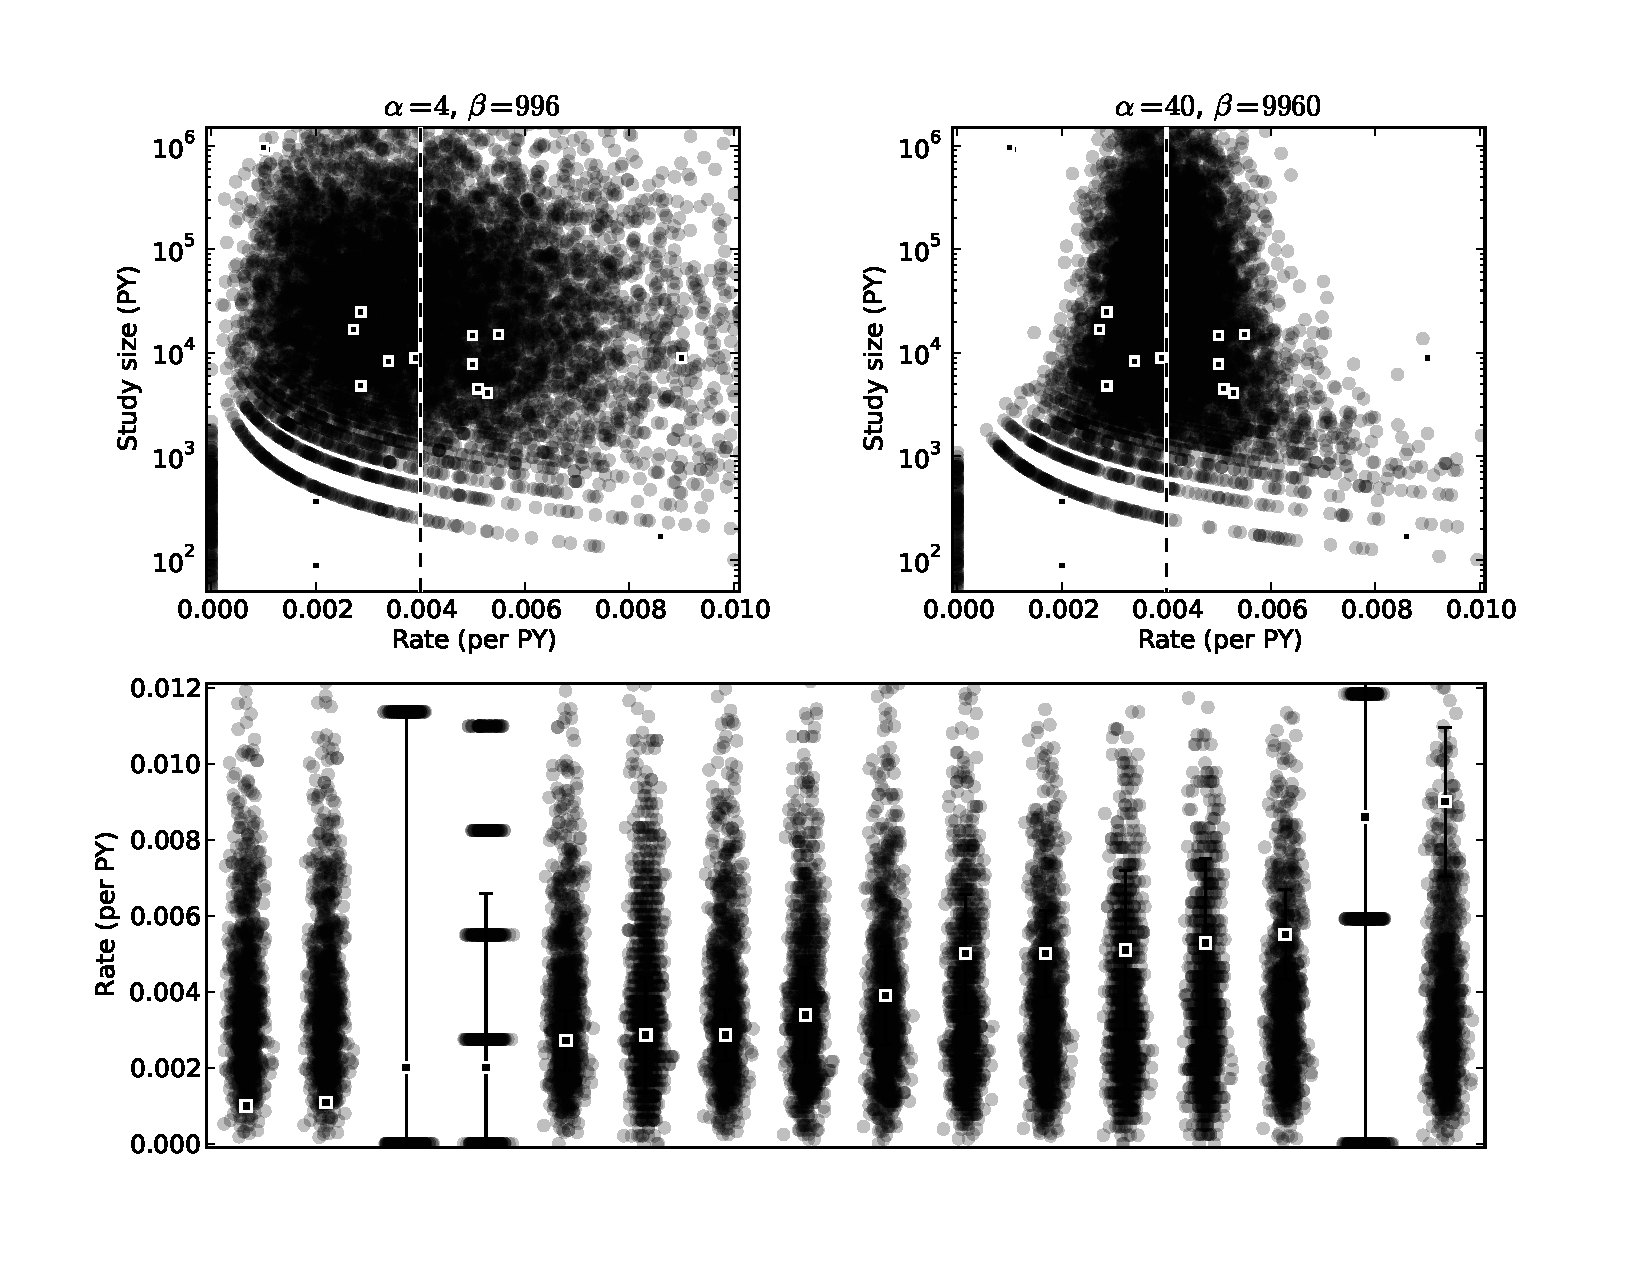
\includegraphics[width=\textwidth]{beta-binomial-funnel.pdf}
\end{center}
\caption{Funnel plot and posterior predictive check for beta binomial
  model. This model captures the heterogeneity in the observed data
  more faithfully than the binomial model from the previous section.
  However, the estimation procedure requires introducing a latent
  parameter for each data observation, and integrating out these
  latent variables is too computationally demanding to be feasible in
  many current applications.}
\label{rate-model-beta-binomial-funnel}
\end{figure}

This model addresses the theoretical shortcoming raised in the
previous section: if studies of $50,000$ people show prevalences of
$2$ and $6$ per thousand, then the posterior distribution of the beta
binomial model has mean $4$ with 95\% HPD interval $[1,8]$, which
seems quite reasonable.

The great shortcoming of the beta-binomial model is computational.
There is no closed-form solution to the integral in the probability
density for the beta binomial model.  Evaluating it requires
introducing a latent variable for each of the data points in the
likelihood.  This simply had too much cost for the numerical
algorithms and computational infrastructure available.

\section{Poission model}
There are two traditional approximations to the binomial distribution,
depending on how large $k$ is in relation to $n$.  When $k/n$ is
large, the normal distribution is used, and when $k/n$ is small, the
binomial is similar to the Poisson distribution.

Since I expect to usually be in a ``small $k/n$'' setting, I will not
develop the normal model in detail now, although in the next section I
will develop the model based on monotonic transformations of the
normal distribution which include a normal model as a special case.

The Poisson distribution is given by the equation
\[
\Pr[X=k] =
\frac{\lambda^k e^{-\lambda}}{k!},
\]
and it can be understood intuitively as the number of times a
``memoryless'' event occurs in a unit time period.  Setting $\lambda
=\pi n$ produces an approximation to the binomial distribution, which
is quite accurate for large $n$ and small
$k$. Figure~\ref{rate-model-poisson-approx-to-binom} demonstrates how
precise this approximation can be when approximating a binomial
distribution with $n=500$ and $\pi=\frac{1}{40}$.

\begin{figure}[h]
\begin{center}
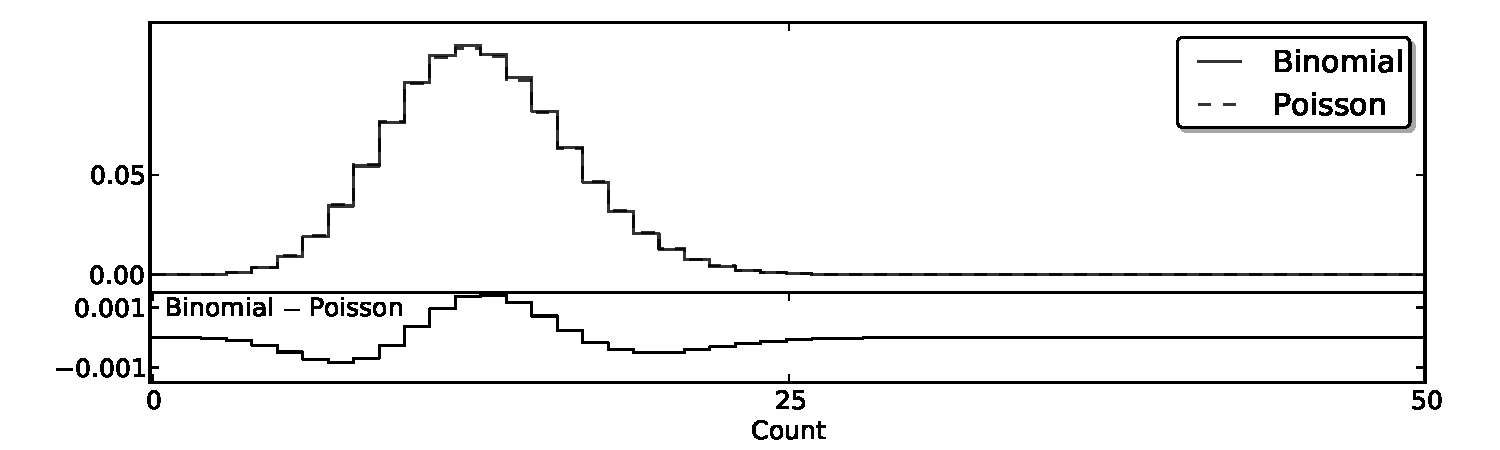
\includegraphics[width=\textwidth]{poisson_approx_to_binom.pdf}
\end{center}
\caption{The Poisson distribution approximates the binomial
  distribution very closely. Here a binomial distribution with $n=500$
  and $\pi=\frac{1}{40}$ is approximated by a Poisson distribution
  with parameter $\lambda=\frac{25}{2}$.  The difference between the
  distributions is shown in the lower panel, since the curves in the
  upper panel are almost indistinguishable by eye.}
\label{rate-model-poisson-approx-to-binom}
\end{figure}

Because of the similarity of these distributions, my Poisson model,
which is defined as
\[
\dens(r\given \pi,n) \propto (\pi n)^{\lfloor
  rn\rfloor} e^{-\pi n},
\]
is quite similar to the binomial model defined above.  It is also
subject to all of the concerns raised about the binomial model
regarding inappropriately low levels of uncertainty when modeling
rates with non-sampling variation at the level typically gathered in
systematic review.

There is one key benefit to this model, compared to the binomial and
beta-binomial models, however.  The Poisson model assigns a
theoretically justified and non-zero likelihood to rates of more than
one.  Although prevalence is always less than one, it is theoretically
possible to have incidence rates more than one, and remission rates
are often more than one (per person-year).


\section{Negative Binomial Model}
Another benefit from the count model approach is to be found in the
Poisson model's over-dispersed cousin.  This distribution is called
the negative binomial distribution (named after the formula that
proves it does indeed sum to one).  Unlike the beta-binomial
distribution, it \emph{does} have a closed form (if you consider the
gamma function ``closed''):
\[
\Pr[X = k\given \pi, \delta] =
 \frac{\Gamma(k+\delta)}{\Gamma(\delta)k!} \left(\frac{\delta}{\pi+\delta}\right)^\delta \left(\frac{\pi}{\pi+\delta}\right)^k
\]

However, this closed form obscures the intuition behind the negative
binomial distribution, which is quite similar to the intuition behind
the beta-binomial distribution (but less clear from its name). Through
a bit of algebra, the negative binomial distribution can be
represented as a hierarchical model, where the observed data comes
from a Poisson distribution, and the parameter of the Poisson
distribution is itself a random variable that comes from a gamma
distribution:
\begin{align*}
X\given \pi &\sim \Poisson(\pi)\\
\pi &\sim \GammaDist(\mu, \delta)
\end{align*}

Here the Gamma distribution is defined by (TK reparameterize to match above)
\[
\dens(x; k,\theta) = x^{k-1} \frac{e^{-x/\theta}}{\theta^k \, \Gamma(k)}.
\]
Through this lens, the negative binomial model can be interpreted as a
natural adaptation of the traditional random effects model in linear
regression to the Poisson case, where each observation comes from a
different Poisson model and the Poisson parameter of these models are
all drawn from a common Gamma distribution. Thus a rate model based on
this distribution provides benefits in handling non-sampling variation
similar to those demonstrated for the beta binomial distribution
above, but in a formulation that is much less demanding
computationally.  The negative-binomial rate model for observing a
rate of $r$ in a population of size $n$ is:
\[
\dens(r\given \pi, \rho, n) \propto
 \frac{\Gamma(\lfloor rn\rfloor+\rho)}{\Gamma(\rho)} (1-\pi)^\rho \pi^{rn}.
\]

Figure~\ref{rate-model-negative-binomial-funnel} shows funnel plots
for two levels of over-dispersion, as well as the posterior predictive
distribution for the negative binomial model.

\begin{figure}[ht]
\begin{center}
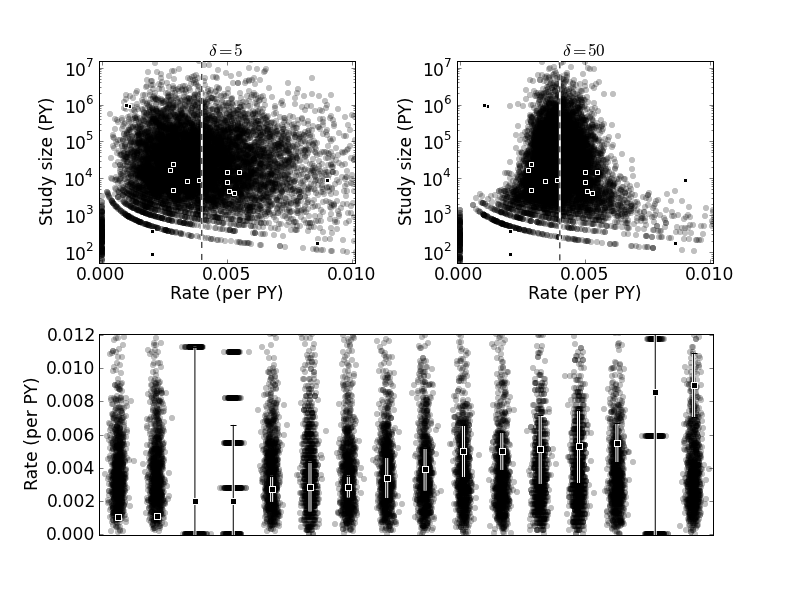
\includegraphics[width=\textwidth]{negative-binomial-funnel.png}

\end{center}
\caption{Funnel plot and posterior predictive check for negative
  binomial model. More description
  TK.} \label{rate-model-negative-binomial-funnel}
\end{figure}

TK discussions of challenges in negative binomial model convergence,
alternative approach based on modeling the ``design effect''
explicitly.

\section{Transformed normal models}
\label{transformed-normal-models}
Some epidemiological data is not count data at all.  Duration studies
and studies measuring the relative risk of mortality are two that come
up frequently in systematic review.  For duration data, a normal model
is sufficient, and a log-normal model proves to be appropriate for
modeling relative risk data, which can be thought of as a ratio of
count variables.

Transformed normal models have also been used for mortality rates in
the past \cite{Girotsis and King-Demographic Forecasting Book}, and
are worthy of continued consideration for modeling the incidence,
prevalence, remission, and mortality as an alternative to the negative
binomial.

In this section, I will develop a general transformed normal model,
and compare it to the negative binomial model.  The adjective
``transformed'' refers to a function which I will keep quite general
for now, requiring it only to be increasing and differentiable,
i.e. for any $x > y$ the transformation $f$ must have $f(x) > f(y)$
and $f'(x)$ must be defined.  Then the transformed normal model will
be derived from the normal distribution, defined by the probability
density
\[
\dens(x\given \pi, \sigma)
 \propto \frac{1}{\sigma}
\exp\left\{ -\frac{(x-\pi)^2}{2\sigma^2} \right\}.
\]

For any increasing, differentiable function $f$, this distribution can
be converted to an $f$-transformed normal model with probability
density
\[
\dens(r \given \pi, \sigma, f, s) \propto
\exp\left\{-\frac{\left(f(r)-f(\pi)\right)^2}{2\left((sf'(r))^2+\sigma^2\right)}\right\},
\]
where $s$ is the standard error of the rate $r$, which is more
convenient that the effective sample size $n$ in this case. The
denominator of the exponent deserves some additional discussion.  For
the identity function $f(x) = x$, the derivative $f'(x) = 1$, and the
denominator simplifies to $2(s^2 + \sigma^2)$, a familiar ``inverse
variance'' weighting where $\sigma$ is a random effect to account for
over-dispersion.  When $f$ is a more complicated function, the term
$sf'(r)$ approximates the standard error of the transformed value
$f(r)$.  Although more sophisticated approximations are possible,
experience dictates that the non-sampling variation (parameterized by
$\sigma$) is always larger than the chance variation, so a simple
approximation of the chance variation is sufficient.

Some common transformations $f$ used in related work yield the
lognormal model ($f(x) = \log x$) the logit model ($f(x) = \logit x$)
and the probit model ($f(x) = \probit x$).  All of these approaches
have a significant drawback, however.  The transformation is not
defined for $x=0$, so these models cannot use data showing rates of
zero. There are two common methods to fix this, dropping all zeros,
and adding a small offset.  Dropping measurements of zero is clearly
problematic, as it leads to systematic bias in the data that remains
and produces estimates larger than the truth.  This is especially
problematic for high quality studies which focus on the age pattern of
a disease, where it is quite reasonable for some age groups to have
zero cases observed.  The effect of dropping zeros is to overestimate
the rates in these age groups.

Adding a small amount, such as $0.5$ is an alternative solution, and
indeed, this is the approach taken for cause-specific mortality
estimation in \cite{Girotsis King-Demographic Forecasting}.  The
selection of the offset can appear ad hoc, however.

Within the framework of the transformed normal model, there is room to
put the solution on firm theoretical foundations.  For example, by
taking $f_\zeta(x) = \log(x + \zeta)$, I obtain the ``offset log
transformed model'', which does allow rates of zero, simply by taking
a positive value for $\zeta$.  This model will not be used extensively
in the example application to come later in this book, but it seems
like a promising approach.  It is particularly appealing in the way it
decomposes the sampling variation into an additive error $\zeta$ and a
multiplicative error $\sigma$, and I expect that it will prove useful
in the future.  For completeness, here is the probability density for
the offset log transformed model:
\[
\dens(r\given \pi, \sigma,\zeta, s)
\propto \exp\left\{
-\frac{\left(\log(r+\zeta)-\log(\pi+\zeta)\right)^2}
      {2\left(\left(\frac{s}{r+\zeta}\right)^2+\sigma^2\right)}
\right\}.
\]

\section{Lower-bound data model}
Cause-specific mortality rates are a special case among the
epidemiological rates available for integrative systems modeling of
disease in a population.  These data come from careful processing of
vital registration system outputs, from verbal autopsy studies, and
from some other sources. But unlike incidence, prevalence, and
remission data, there is no rate or ratio in the compartmental model
that corresponds directly to this quantity.  This is because of the
``one death has one cause'' mantra of biomedical theory.  The excess
mortality rate in the system dynamics model from Chapter TK is not
entirely compatible with this idea.

Cause-specific mortality data nonetheless provides \emph{some}
information, and should be used in an integrative model if it is
available, especially if other sources are sparse and noisy, (which
they always are, in my experience).  By decomposing the excess
mortality into part that is ``cause-of-death mortality'' and residual
excess mortality, i.e. $f = f_{cod} + f_{non}$, it follows that $\CSMR
=p \cdot f_{cod} \leq p\cdot f$, so the following lower bound model is
appropriate:
\[
\dens(\CSMR \given \pi,\delta) =
\begin{cases}
  \calD(\CSMR, \pi, \delta), &\qquad\text{if } \pi-\CSMR \geq 0;\\
  \calD(\pi, \pi, \delta), &\qquad\text{otherwise.}
\end{cases} 
\]

\section{Data values of zero}
Rates with measured values of zero can present a particular challenge
for some statistical models, and are worthy of careful
investigation. As discussed in Section~\ref{transformed-normal-models}
above, there are a number of ad hoc approaches that have been
developed to allow data that includes rates of zero to be fit in
models that do not allow zero rates explicitly, such as dropping all
of the observations with value zero, or replacing them by a small, but
non-zero value. However, it is clear that these approaches will
introduce bias to the estimates \cite{refs TK}

TK challenges of coming up with effective sample size for data with
value zero found in systematic review, and some potential approaches
for addressing this, including the failed approach of using the
standard error from the normal approximation to the binomial.

Fortunately, all of the count models described above allow data with
zero values to be included without requiring an ad hoc
modification. Figure~\ref{zero-forest} shows how all of these models
perform for a simulated data set of prevalence data for a rare
condition that has population prevalence of $1$ in $10,000$.  Since
the simulated studies of this disease range in sample size from
$n=2,500$ to $n=400,000$, it is expected that some of the smaller
studies will find no individuals with the condition. To make things
even harder for the models, I have ``inflated'' the number of zero
studies, by deterministically including $4$ studies which measured
prevalence levels of zero.

A statistical model with appealing theoretical foundations that
explicitly models this ``zero-inflation'' phenomenon is the
zero-inflated beta binomial model, which is even less efficient than
the beta binomial model that was considered in
Section~\ref{beta-binomial-model}.  It augments the beta binomial
model with an additional parameter $\phi$, and uses a mixture
likelihood where each rate has value $0$ with probability $\phi$ and
value given by a beta binomial distribution (which may also have value
$0$) with probability $1-\phi$.

Formally, the zero-inflated beta binomial distribution is defined
by
\begin{align*}
&\dens(r\given \alpha, \beta, \phi, n)\\
&\propto\quad\begin{cases}
  (1-\phi)\int_{\pi} \pi^{\alpha-1}(1-\pi)^{\beta-1} \pi^{\lfloor
    rn\rfloor} (1-\pi)^{\lceil (1-r)n\rceil} d\pi, &\quad\text{if } r > 0; \\
  \phi + (1-\phi)\int_{\pi} \pi^{\alpha-1}(1-\pi)^{\beta-1}
  (1-\pi)^{n} d\pi, &\quad\text{if } r = 0.
\end{cases}
\end{align*}

\begin{figure}
\includegraphics[width=\textwidth]{zero_forest.pdf}
\caption{Forest plot comparing models fit to simulated data for a rare
  disease.  The simulation inflated the number of observed zeros to
  challenge the models.}
\label{zero-forest}
\end{figure}

\section{Summary and Comparison}
This section has developed $7$ alternative rate models, all with
benefits and drawbacks.  The binomial model is simple and
theoretically appealing, but does not handle non-sampling variation,
producing over-confident estimates in the face of noisy data.  The
beta binomial model deals with over-dispersion through a theoretically
appealing extension to the binomial model, but it is too
computationally demanding to use in my applications.  The Poisson
model is a close approximation to the binomial model, and has all of
the drawbacks except it can handle rates greater than 1, which is
important for modeling remission rates.  So it is the negative
binomial model, which extends the Poisson model analogously to the way
the beta binomial model extends the binomial model that I have settled
on for most of the applications to follow, using it to model
incidence, prevalence, remission, excess-mortality, and cause-specific
mortality. It is not as amenable to analysis as I would like however,
and sometimes benefits from weakly informative priors on the
over-dispersion parameter, an undesirable feature that slows down
analysis by requiring sensitivity analysis.  Transformed normal models
are a promising alternative approach, and I have used the normal model
for duration data in some of the following examples, as well as the
lognormal model for standardized mortality rate data and relative
mortality risk data. The offset log transformed model seems
particularly promising as an alternative to the negative binomial
model, and understanding its statistical and computational
characteristics is a promising direction for future research.

TK some sort of comparison: simulation study? posterior predictive
checks? something analogous to SMART counties in small areas
estimation?
